\documentclass[article,twocolumn,preprint,10pt]{paper}%{revtex4-1}
\usepackage{epsfig,graphicx,amsmath}
\usepackage{amsfonts,amssymb,amsthm}
\usepackage{enumerate}
\usepackage{epstopdf}
\usepackage{afterpage}
\usepackage{color}
\usepackage[many]{tcolorbox}

\usepackage[caption=false]{subfig}
\newcommand{\nn}{\nonumber}
\newcommand{\ba}{\bea \begin{array}}
\newcommand{\ea}{\end{array} \eea}
\renewcommand{\(}{\left(}
\renewcommand{\)}{\right)}
\renewcommand{\[}{\left[}
\renewcommand{\]}{\right]}
\newcommand{\bc}{\begin{center}}
\newcommand{\ec}{\end{center}}
\newcommand{\p}{\partial}
\newcommand{\cb}{\mbox{\boldmath$c$}}

\newcommand{\red}{\textcolor{red}}
\newcommand{\blue}{\textcolor{blue}}
\newcommand{\mb}[1]{ \mbox{\boldmath$#1$}}
\newcommand{\ds}{\displaystyle}
\newcommand{\beq}{\begin{eqnarray}}
\newcommand{\eeq}{\end{eqnarray}}
\newcommand{\beqq}{\begin{eqnarray*}}
\newcommand{\eeqq}{\end{eqnarray*}}
\newtheorem{thm}{Theorem}[section]


\usepackage{rotating}
\newcommand{\g}{\gamma}
\newcommand{\epsv}{\epsilon}
\newcommand{\eps}{\varepsilon}
\newcommand{\oln}{\overline }

\newcommand{\Om}{\mbox{\boldmath$\omega$}}
\newcommand{\x}{\mbox{\boldmath$x$}}
\newcommand{\U}{\mbox{\boldmath$U$}}
\newcommand{\V}{\mbox{\boldmath$V$}}
\newcommand{\R}{\mbox{\boldmath$R$}}
\newcommand{\E}{\mbox{\boldmath$\eta$}}
\newcommand{\Id}{\mbox{\boldmath$I_d$}}
\newcommand{\M}{\mbox{\boldmath$M$}}
\newcommand{\N}{\mbox{\boldmath$N$}}
\newcommand{\1}{\mbox{\boldmath$1$}}
\newcommand{\hx}{\mbox{$\hat x$}}
\newcommand{\n}{\mbox{\boldmath$n$}}
\newcommand{\J}{\mbox{\boldmath$J$}}
\newcommand{\y}{\mbox{\boldmath$y$}}
\newcommand{\z}{\mbox{\boldmath$z$}}
\newcommand{\bt}{\mbox{\boldmath$\beta$}}
\newcommand{\tb}{\mbox{\boldmath$t$}}
\newcommand{\ic}{\mathtt{i_c}}
\newcommand{\di}{\text{d}}

\font\bb=msbm10 at 12pt \font\bbbis=msbm10 at 10pt
\def\bz{\bar{z}}
\def\rR{\hbox{\bb R}} \def\nN{\hbox{\bb N}}
\def\rRp{\hbox{\bbbis R}} \def\nN{\hbox{\bb N}}
\def\zZ{\hbox{\bb Z}} \def\qQ{\hbox{\bb Q}}
\def\cC{\hbox{\bb C}} \def\sS{\hbox{\bb S}}
\def\pP{\hbox{\bb P}}

\newcommand{\vect}[1]{\boldsymbol{#1}}


%%%%%%%%%%%%%%%%%%%%%%%%%%%%%%%%%%%%%%%%%%
\begin{document}
	%%%%%%%%%%%%%%%%%%%%%%%%%%%%%%%%%%%%%%%%%%
	\title{Machine-learning model for the predicting of subjective spherocylinderical component from objective measurements}
	\author{Ofir Shukron, Jacky Hochner. Michael Assouline MD.\\   Mikajaki}
	
	\maketitle
	\section{Summary}\label{section:Highlights}
	 \begin{itemize}
		\item We trained two Random-Forest classifiers to predict sphero-cylindrical component of the subjective refraction, based on objective measurements from Visionix vx120 refractometer;
		\item We obtain 85\% accuracy of subjective Sphere component within 0.25D range;
		\item We obtain 90\% accuracy of the subjective Cylinder component within 0.25D range;
		\item We obtained $\sim10$\% improvement  over VX120 refratometer in predicting the \textbf{exact} subjective sphere and cylinder (i.e. error =0D);
		\item We obtained $\sim10$\% improvement in accuracy over VX120 in prediction subjective refraction within the error range $0.25D$, and 6-8\% improvement in accuracy over the vx120 for the error range 0.5D;
		\item Overall, we predict both sphere and cylinder simultaneously to within 0.25D of the subjective in 75\% of cases vs. 64\% of the refractometer.
	\end{itemize}
	\section{Introduction}\label{section:Introduction}
	We describe here a procedure of training a machine learning classifier to predict the subjective refraction (sphero-cylinder components) of a patient based on their objective measurements from a refractometer. The process of assigning subjective refraction by trained personal requires 5-10 minutes per patients using a phoropter, after acquiring objective measurements (2-3 minutes). We thus aim here at presenting a model, which reduces or completely eliminates the need for subjective refraction, or at least provides ophthalmologist with a starting point closer to the subjective refraction values, thus reducing th overall examination time.
	
	The problem of assigning subjective refraction based on objective measurement is a long lasting challenge. Various factors affect the precision and repeatability of the subjective refraction\cite{elliott1997}. 
	Intra-operator variability of the subjective refraction, and can range in 95\% limits of agreement to  $\pm0.94D$ for cycloplegic subject to $\pm0.64$ for non-cycloplegic subjects \cite{zadnik1992}, whereas Inter-operator variability was also reported to reach $\pm0.29D$ \cite{bullimore1998,raasch1998} within 95\% limits of agreement. Differences between the autorefractometer and subjective are also well known for cases of astigmatism and large ametropia \cite{thompson1996}. However some authors report that no significant difference exist between autorefractometer and subjective refraction \cite{bennett2015}, which might indicate a dependence on subjective refraction assignment methodology in the clinics. Variability between accuracy and quality of the ophthalmic machine can also enlarge the difference between the objective and final subjective, with a difference ranging between 0.16 to 0.5D \cite{kumar2021}, or a tendency of the sensors toward assigning hyperopic refraction \cite{choong2006}. Finally, underlying conditions such as keratoconus can hamper repeatability of subjective refraction to within 4-6 times larger difference than with regular myopic \cite{raasch2001}.
	
	Models for the prediction of refraction errors have been previously attempted by several authors using various methodologies and acquisition machinery. Measurement from wavefront aberrometers were used in \cite{guirao2003}, who demonstrated the contribution of high order aberrations (HOA) to refractive errors using an optimization routine, which predicts the sphere and cylinder best suited to optimize image quality on the retinal plane. Results show 0.4D error for the sphere and 0.2D for the cylinder on a cohort of 146 eyes.
	
	Machine learning methodologies have been applied recently based on measurements from wavefront aberrometers. Three gradient boosted trees models were trained in \cite{rampat2020} on the power vectors of the components of refraction ($J0,J24$, and Spherical equivalent) to yield a mean absolute error (MAE) of 0.12, 0.094, and 0.3 on the three components, respectively. Prediction of the power vector components was also attempted in \cite{leube2019} by a artificial deep learning network, using 36 Zerrnike coefficients as features, and achieved a mean accuracy of 0.08D with 0.78D confidence interval. A random forest classifier was trained in \cite{de2020} on a larger cohort of demographic and ophthalmic data to predict the components of the power vector, and achieved a mean absolute error of 0.33.  Deep learning models were also applied to fundus images to predict the refractive errors \cite{varadarajan2018} and obtained a mean absolute error of 0.56D. Deep convolutional network models were trained  \cite{chun2020} based on images acquired by smartphone and achieved 85\% accuracy in predicting refraction. Despite those models achieving good results, the complexity of data preparation, training and the amount of data needed for reliable training, provides a bottle neck in their usability. 
	
    In this report, we present a simple methodology to train two classifier directly from the measurements of the refractometer to predict the subjective refraction. We show that our result can surpass not only the prediction of the refractometer but also are in par and exceed the accuracy of existing models in the literature. Our initial model forms the basis for further exploration of the feature space, feature design, and model construction, and shows an encouraging approach which allows further improvements.
	\subsection{General methodology}\label{subsection:GeneralMethodology}
	Here we concentrate on predicting the subjective sphere $S_s$ and subjective cylinder $C_s$ components of the refraction based on objective measurements. However, instead of directly predicting $S_s$ and $C_s$, we predict the difference between the objective and subjective sphere and cylinder  $S_o, C_o$ i.e. we aim at predicting the $\Delta$ sets
	\beq 
	\Delta S &=& S_s-S_o,\\
	\Delta C &=& C_s-S_0,
	\eeq
	The $\Delta$ sets are in intervals of 0.25D. 
	We train two independent classifiers to predict the $\Delta S$ and $\Delta C$. Using the predicted $\Delta S$ and $\Delta C$, we  adjust $S_o$ and $C_o$ to obtain the newly predicted subjective $S_s$ and $C_s$, such that $C_s = C_o+\Delta S$ and $S_s=S_o+\Delta S$, whereas we keep the cylinder axis as the one received from the refractometer. 
		
	Predicting the $\Delta$ rather than directly $S_s$ and $C_s$ allows us to predict a larger subjective cylinder and sphere groups, which also helps us overcome limitation of insufficient data to directly predict the subjective refraction.
	The underlying assumption in predicting $\Delta S,\Delta C$ is that observation with similar delta behave similarly. This assumption has no immediate prior justification. 
	
	\section{Results}
	\subsection{Training validation and feature importance}
	We use a dataset of 9763 eye (see Material and Methods \ref{section:MaterialAndMethods}) to train two independent Random Forest (RF), as described in \ref{subsection:trainingAndFeatureDesign}. The inclusion range of $\Delta C$ and $\Delta S$ were chosen such that at least 100 observations were included in each class in the training set (see \ref{subsection:ClassAssignment}). We encode $\Delta S, \Delta C$ sets to class numbers as described in \ref{subsection:ClassAssignment}. A flowchart of the process of feature selection, cross-validation, hyper-parameter tuning, training and validation is depicted in the Material and Methods section \ref{section:MaterialAndMethods}, Fig. \ref{fig:trainvalidationflowautoref}. For the validation of our result we use $\sim 10 \%$ of the data. 
	
	After automatic feature selection, the two resulting RF models for $\Delta S$ and $\Delta C$ included 21 and 19 features, respectively. The full list of selected features appear in the Appendix subsection \ref{subsection:featuresSelected}. The three most contributing features to predict $\Delta S$ were the age, $J0$ and the Zernike coefficient $Z_4^0$. For $\Delta C$ we find the objective cylinder $C_o$, age and the power vector component $J0=-0.5C\cos(2A)$ (see Material and Methods) as the three most contributing features. In Fig. \ref{fig:featureIMportance}  we report the relative importance of the selected features for the $\Delta S$ and $\Delta C$ classifiers within the context of each RF model. The average $\Delta S$ tended to increase with age, whereas $\Delta C$ decreased with age (see Fig. \ref{fig:dSdCvsAge}), which might indicate the limitation of the refractometer to accurately capture the refraction in the elderly population. The $J0$ component of the power vector showed symmetric correlation around the zero value for $\Delta S$ with tendency to decrease for $J0\geq 0$ and increase for $J0\leq0$, whereas the average $\Delta C$ showed inverted trends (Fig \ref{fig:dSdCvsJ0}).
	\begin{figure}[h!]
		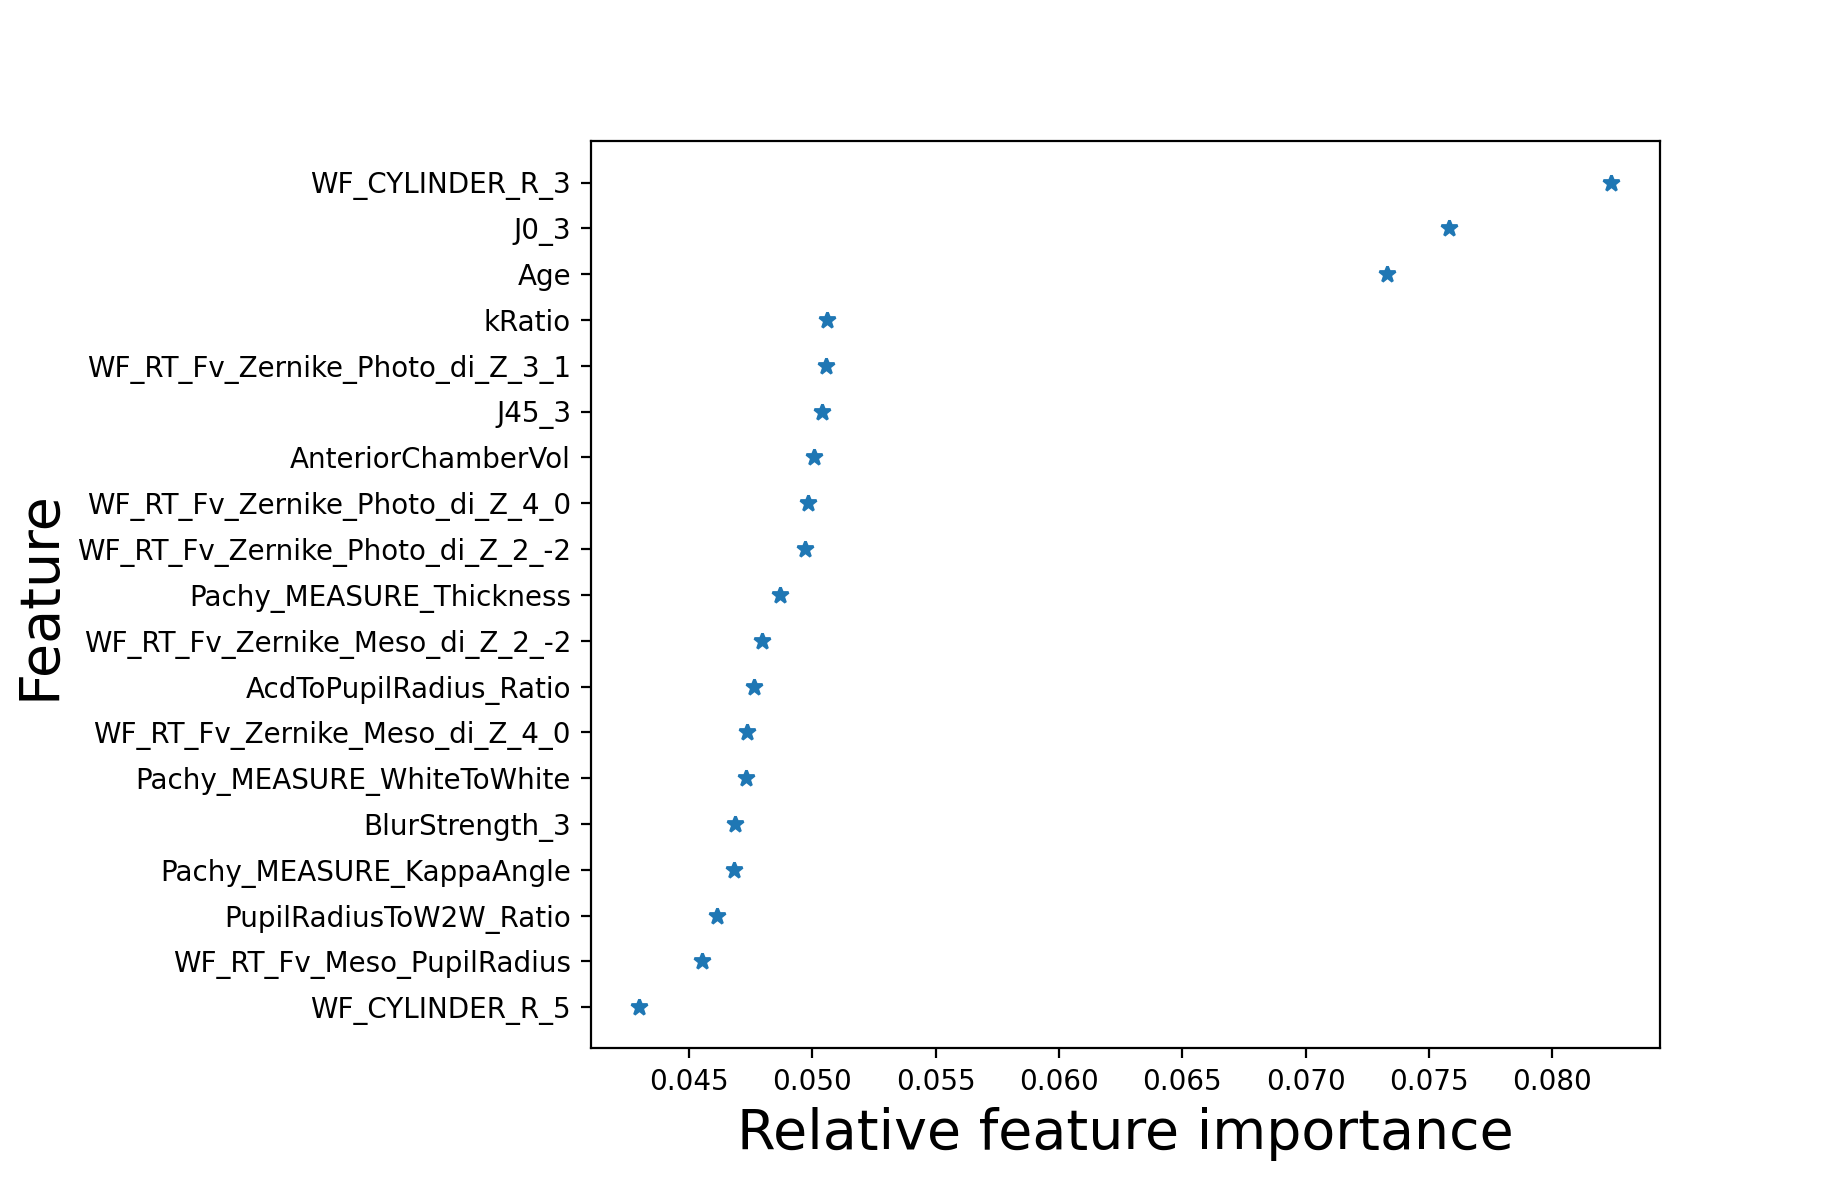
\includegraphics[width=1\linewidth]{featureImportanceCylinder.png}
		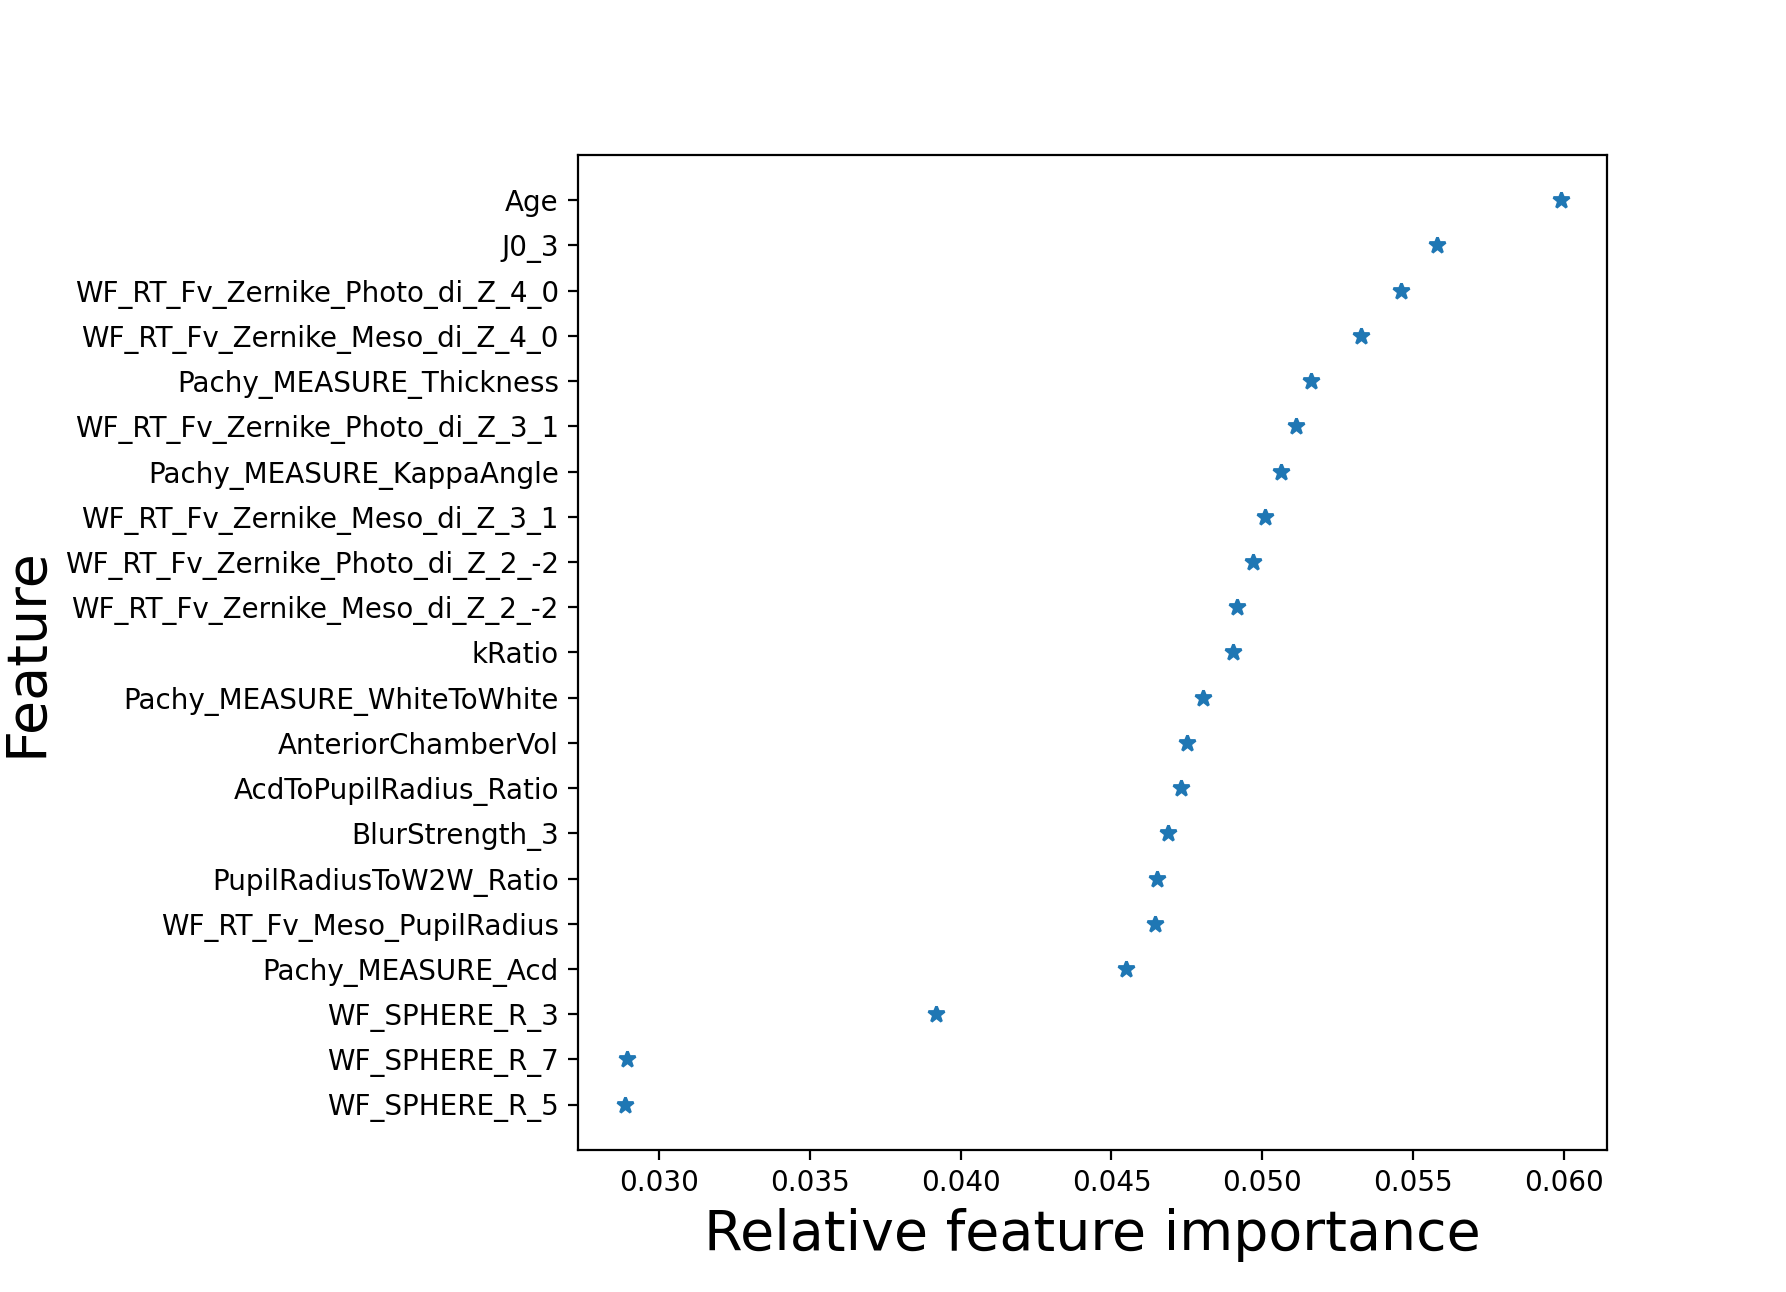
\includegraphics[width=1\linewidth]{featureImportanceSphere.png}
		\caption{Relative contribution of selected features for the Cylinder (top) and Sphere (bottom) predictors within the context of the RF model. Features were automatically selected by model-based feature selection method}
		\label{fig:featureIMportance}
	\end{figure}
	\begin{figure}[h!]
		\includegraphics[width=1\linewidth]{dSVsAge}
		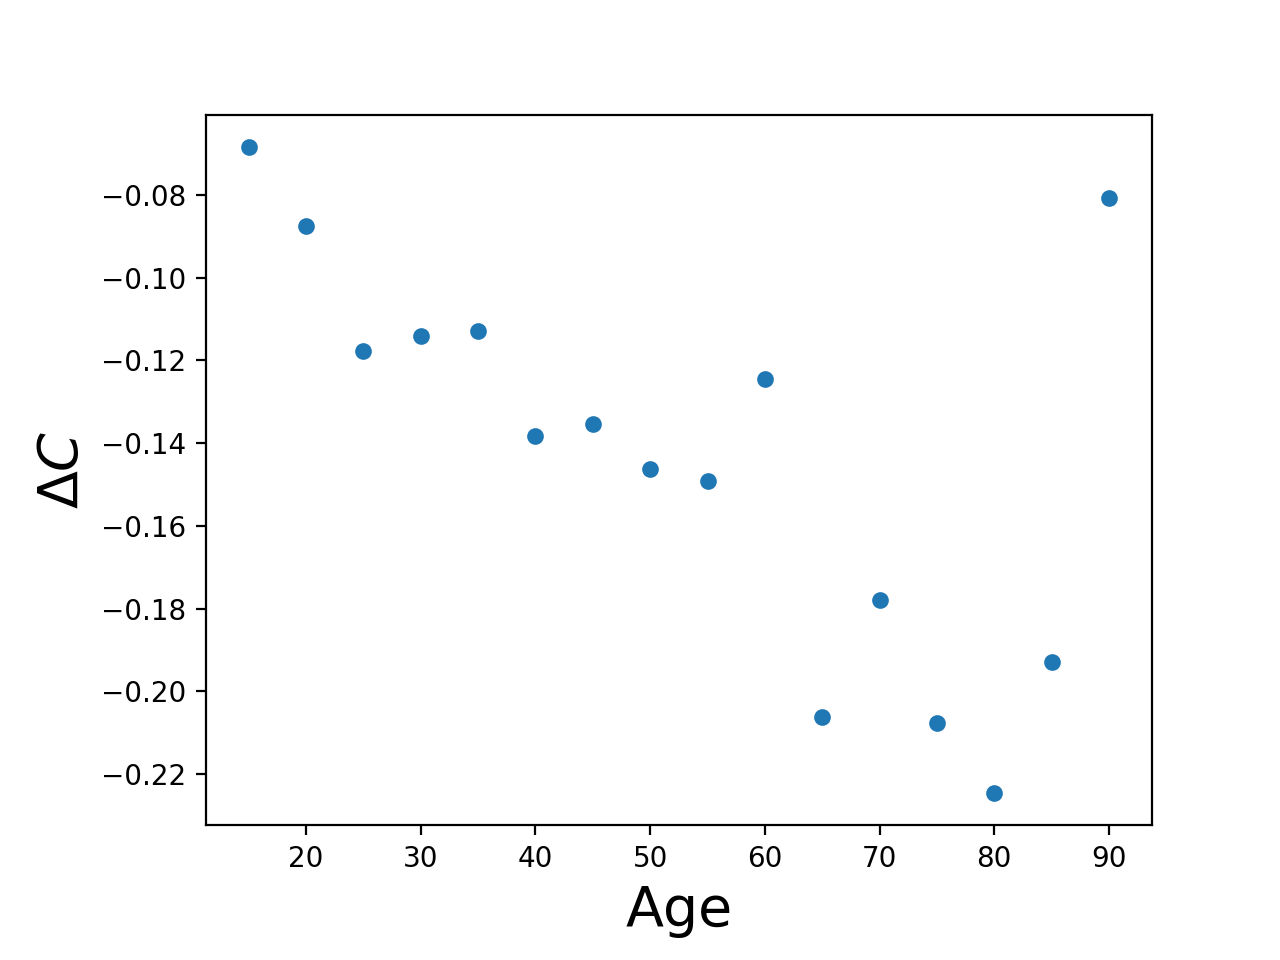
\includegraphics[width=1\linewidth]{dCvsAge}
		\caption{Correlation between age groups and the average $\Delta S$ (top) and average $\Delta C$ (bottom).}
		\label{fig:dSdCvsAge}
	\end{figure}
   \begin{figure}[h!]
   	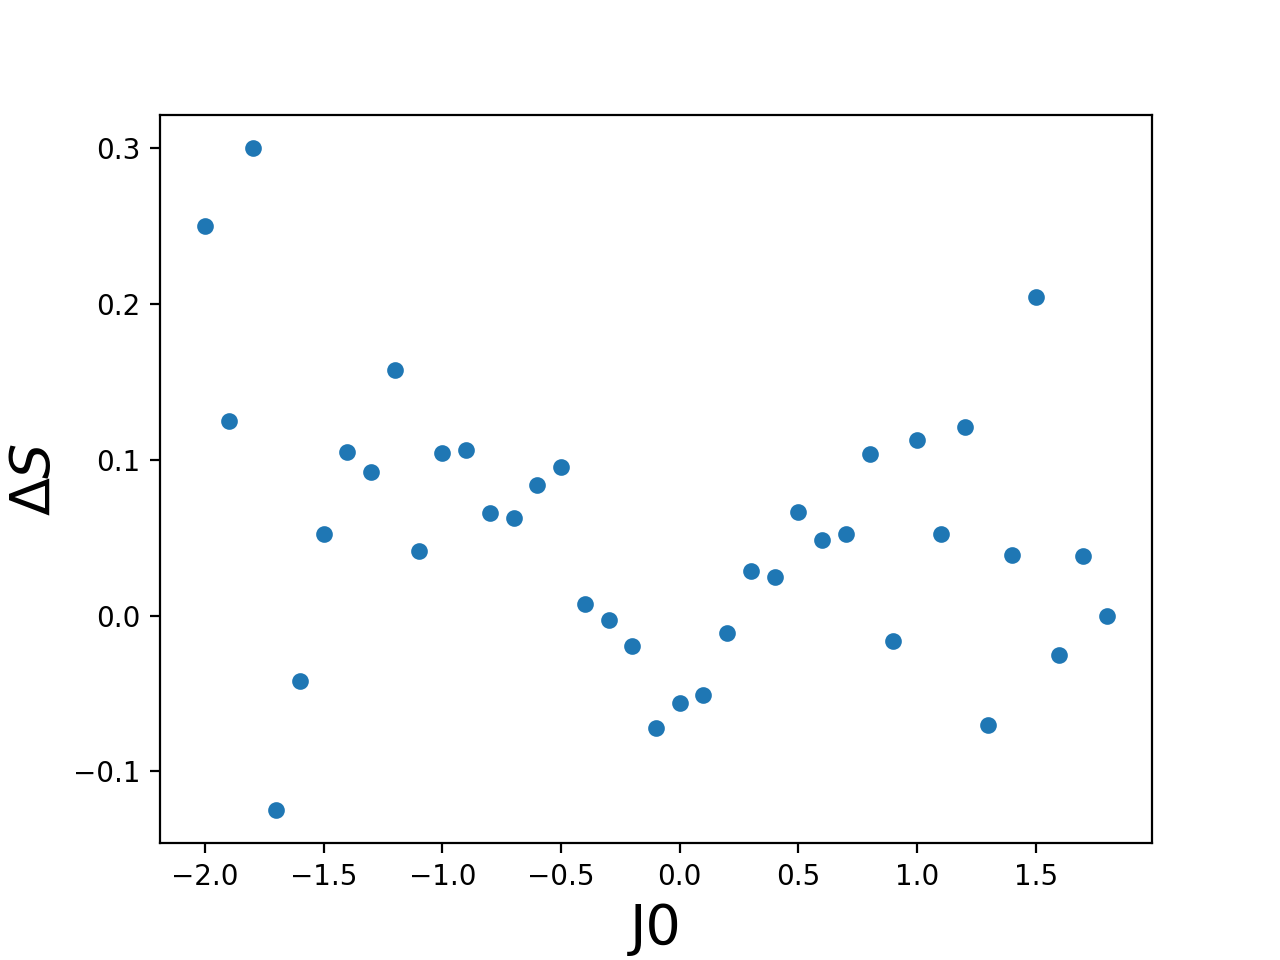
\includegraphics[width=1\linewidth]{dSvsJ0}
   	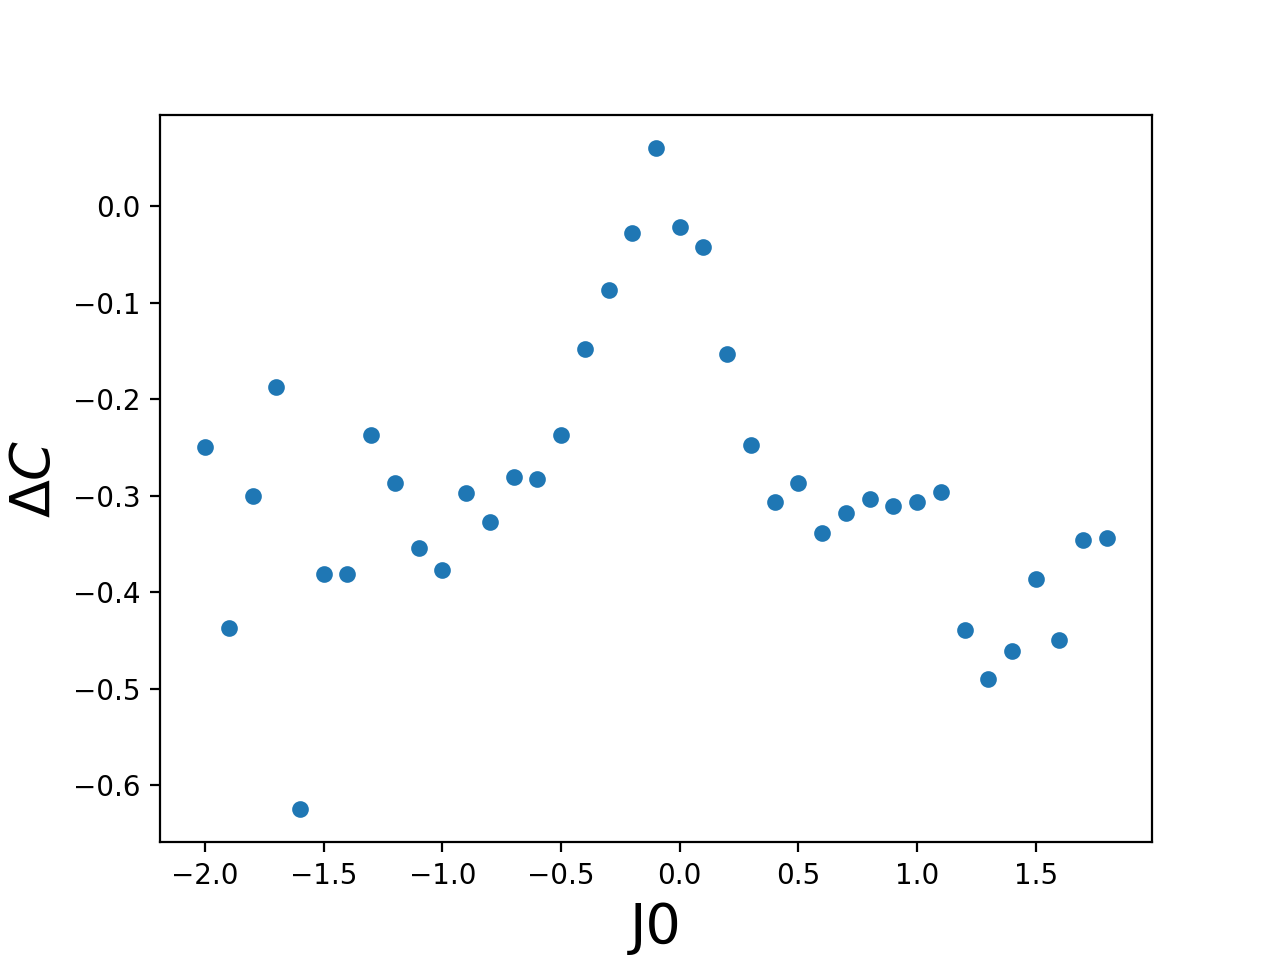
\includegraphics[width=1\linewidth]{dCvsJ0}
   	\label{fig:dSdCvsJ0}
   	\caption{Correlation between the $J0$ component of the power vector (see Material and Methods) and the average $\Delta S$ (top) and average $\Delta C$ (bottom).}
   \end{figure}

	\subsection{Predicting subjective refraction}\label{subsection:PredictingSubjectiveRefraction}
	 In Table \ref{table:resultsCylinderDelta} we report the result of predicting the \textit{exact} subjective refraction (i.e. $\Delta S=0$, $\Delta C=0$) and prediction within the error ranges of 0.25D and 0.5D from subjective refraction. The values of predicted subjective $S$ and $C$ were obtained by adding the predicted $\Delta S$, $\Delta C$ to the objective data, as described in \ref{subsection:GeneralMethodology}. For the $\Delta S$, we obtain 6\% improvement of the exact prediction over the refractometer (36\% refractometer vs 42\% model), and 8\% improvement in predicting within the range of 0.25D (76\% refractometer vs 85\% model).  For $\Delta C$, we obtain 11\% improvement over the refractometer in predicting the exact subjective refraction (35\% refractometer vs 46\% model) and 12\% in prediction within the error range of 0.25D (80\% refractometer vs 92\% model). 
		
	\begin{table}[http!]
		\begin{tabular}{c|c|c|}
			$|\Delta S|\leq\delta$  (D) & Refractometer (\%) & Model (\%)\\
			\hline    
			0       & 36    & \textbf{42} \\
			0.25  & 76    & \textbf{84} \\
			0.5    & 92    & \textbf{96} \\
			\hline
			MAE  & 0.25 & \textbf{0.2} 
		\end{tabular}
		\caption{Summary of results (accuracy \%) of classification of the $\Delta S$ into 9 classes representing $\Delta S$ in the range $[-1,1]D$ with 0.25D intervals, to within an error range of $\delta\in[0,0.25,0.5]$, vs. objective values (vx120 refractometer), and the mean absolute error (MAE).}
		\label{table:resultsSphereDelta}
	\end{table}
	\begin{table}[h!]
		\begin{tabular}{c|c|c|}
			$|\Delta C|\leq\delta$ (D) & Refractometer (\%) & Model (\%) \\
			\hline 
			0          & 35  &  \textbf{46} \\
			0.25     & 80  & \textbf{92} \\
			0.5       & 95  & \textbf{98} \\
			\hline
			MAE     & 0.25  & \textbf{0.22}
		\end{tabular}
		\caption{Summary of result (accuracy \%) of prediction of the $\Delta C$  from 7  classes in the range [-1, 0.5]D with 0.25D intervals to within an error range of $\delta\in[0,0.25,0.5]D$, using a trained RF classifier (Model) vs. objective measurements (vx120) and the mean absolute error (MAE).}
		\label{table:resultsCylinderDelta}
	\end{table}
	We then examining the accuracy of our predictor for simultaneous prediction of $|\Delta S|,|\Delta C|$ to for the \textit{exact} subjective refraction and within an error range of 0.25 and 0.5D. Our classifier achieved 19\% accuracy for the \textit{exact} prediction simultaneously for both components  vs. 14\% for the autorefractometer. In the error range of 0.25D, our predictor achieved simultaneous $|\Delta S|, |\Delta C|\leq 0.25$ for 75\% of the observations vs. 64\% for the refractometer, and 95\% (model) vs. 98\% (refractometer) within the 0.5D error range.  An  error of 0.25D is unnoticeable for patients and is considered a precise subjective refraction, although evidence show  that as low as 0.125D can be detected \cite{marinrefraction}. This result indicate that after our prediction, 3/4 of patient do not need further adjustment to the phoropter to arrive at subjective refraction, vs. 64\% in the refractometer. Thus, we show that using our prediction as a starting point for subjective refraction, the time spent in the phoropter can substantially be reduced. The reminder of 25\% of patient who do need adjustment for their refraction values after our prediction are within an average error range of 0.5D for the $\Delta C$ and within an average of 0.25D for $\Delta S$. 

	\begin{table}
		\begin{tabular}{c|c|c|}
			$|\Delta S|\,|\Delta C|\leq\delta$(D) & Refractometer(\%) & Model(\%)\\
			\hline 
			0              & 14 & \textbf{19} \\
			0.25         & 64 & \textbf{75} \\
			0.5           & 92 & \textbf{95} \\
		\end{tabular}
		\caption{Summary of results (accuracy \%) of prediction both $\Delta S$ and $\Delta C$  to the exact subjective values and within an error range of $\delta \in[0.25,0.5]$, by the RF classifier vs. objective values (vx120 refractometer) for $|\Delta S|, |\Delta C|\leq \delta$, with $\delta\in[0,0.25,0.5]$.}
		\label{table:resultsSphereAndCylinderDelta}
	\end{table}
	
	\section{Discussion}
	In this report we present a machine-learning model to predict subjective sphere and cylinder based on objective VX120 measurements. We demonstrated the superiority of our classifiers in prediction of subjective refraction over VX120, improving the accuracy by $\sim10\%$ in both Cylinder and Sphere components. The vx120 autorefractometer is accurate simultaneously for the exact sphere and cylinder component in only 14\%  and 64\% in the error range of 0.25D, our classifiers reach exact prediction in 19\% of the cases and 75\% within the error range of 0.25D (see Table \ref{table:resultsSphereAndCylinderDelta}). Our results show that, using our method, for 3/4 of patient no further adjustment to the phoropter is needed beyond the predicted values. The remaining 25\% of patient that do need adjustment are within an average error range of 0.5D  for the cylinder component and within 0.25D error in the sphere component. In the process of assigning subjective refraction using a phoropter, our results then translate  to an average of two clicks correction in cylinder component and a single click for the sphere. Hence, our methodology can also provides a starting point for the subjective refraction, closer to the eventual values.  The advantage of automatic prediction of subjective refraction can be seen in places where the autorefractometer doesn't do well enough, i.e. for $|\Delta S|=0$ and $|\Delta_C|\leq 0.25D$ and in the elderly population (see Fig \ref{fig:dSdCvsJ0}).
	
   Our approach at training and validation differs from previous machine learning models, constructed by other authors, which attempts at either predicting directly the components of the subjective refraction or the components of the power vectors ($J0,J45,SE$). We show here that using a simple approach of predicting $\Delta $ and $\Delta C$, we are able to surpass results of predicting the  subjective refraction obtained by these authors, with mean absolute error of prediction of 0.2D. Our predictor is able to capture a wide range of the refractive error ranging from -6D to 5D in the sphere component and -6D to 0 in the cylinder. 
   	
	To summarize, in this short report we demonstrated a simple and promising approach for predicting the sphero-cylindrical components of the subjective refraction. This report should serve as a starting point to further improvement of the model's accuracy, by either collecting more data and re-training the model and by continuous and intelligent feature design.  Future efforts should concentrate on improving classification accuracy within the error bounds of up to 0.25D, where the margin of improvement still remain large (theoretically 20\% for the cylinder and 24\% for the sphere components can be improved, and a joint Sphere-Cylinder improvement of 25\% is attainable).
	 Effort of improvements can equally concentrate on aspects of model selection and training. Here we devised a tailor-made cross-validation function (Eq. \ref{eq:cvScore}), to encourage in the process of iterative model parameter tuning, those parameter sets which produces models with increasing number of predictions within the error range of 0.25D. The interval of 0.25D as an error measure, was chosen to incorporate the knowledge that subjective refraction errors within this range are not detectable by patient, although new evidence now show that 0.125D can also be detected \cite{marinrefraction}. Our CV function score can further be adjusted to include smaller error intervals, given the appropriate data. 
	 
	 Acquisition of additional data can greatly affect the training results and allow us to better predict for classes at the edges of the $\Delta S$ and $\Delta C$ range (e.g. at 1D difference). The distribution of $\Delta S,\Delta C$ across population is non-uniform, with the majority of values in the range of [-0.25,025]D (near 30 folds those at [-1,1]D), whereas observations for $\Delta S, \Delta C=\pm1D$ are relatively rare. The uneven distribution creates limiting factor in the training stage and might result in a bias toward predicting observations to lower $\Delta$ than it should. Equalizing classes in the training set, does not alleviate this issue (data not shown). 
	 
	Lastly, our model will greatly benefit from an addition of a directional predictor, one which provide probabilistic measure to the direction in which the objective sphero-cylindrical component need to be adjusted to arrive at the subjective refraction values. Such a predictive model can be placed prior the classification of the actual $\Delta S, \Delta C$ and therefore its output can be passed on as a feature for further classification. This model is in stages of research and development.
	
	\section{Material and Methods}\label{section:MaterialAndMethods}
	\subsection{Data Preparation}\label{subsection:DataPreparation}
	Data used in this study were contributed by the Prevot clinic, and collected between January 2019 to December 2020 and Clinique Iena Vision, Paris France. Objective measurements were acquired using the Visionix VX120 refractometer  and subjective refraction was performed by trained personnel in the clinic using a phoropter. 
	
	We applied an inclusion criteria for measurements in this study, as described in Table \ref{Table:inclusionCriteria}. 
	\begin{table}
	\begin{tabular}{l|c}
		parameter & range\\
		\hline 
       Age & [15,100]\\	
       ACD & [2,5]\\
       S      & [-5,6]\\
       C      & [-6,0]\\
       $\Delta S$ & [-1,1]\\
       $\Delta C$ & [-1,0.5]\\
       wtw & [8,16]\\
       pachy & [400,600]\\
       angle $\kappa$ & [0,25]
	\end{tabular}
     \caption{Inclusion criteria for patients in this study.}
     \label{Table:inclusionCriteria}
	\end{table}
   After applying the inclusion criteria, our database contained 9763 eye records.
   Missing entries for each measurement were imputed based on median value of the existing feature (column) values. The median was chosen to avoid replacing missing entries by non-valid values (e.g. such as would have obtained by imputing using the mean of each feature). 
   
   \subsection{Class assignment}\label{subsection:ClassAssignment}
   Classes of the $\Delta S$ and $\Delta C$ were encoded to an integer number. Class encoding for sphere and cylinder appear in Table \ref{table:classEncoding}.
   \begin{table}
   	\begin{tabular}{l|c|c}
   		$\Delta$ & $\Delta S$ class & $\Delta C$ class \\
   		\hline 
   		-1        & 0 & 0\\
   		-0.75   & 1  & 1\\
   		-0.5    & 2  & 2\\
   		-0.25  & 3  & 3\\
   		0        & 4   & 4\\
   		0.25   & 5   & 5\\
   		0.5     & 6   & 6\\
   		0.75   & 7    &  \\
   		1        & 8    &  \\
   		\end{tabular}
   	\caption{Encoding of $\Delta S$ and $\Delta C$ into class integer numbers.}
   	\label{table:classEncoding}
   	\end{table}
   
   The number of classes was determined based on the availability of sufficient number of measurements in each delta set. We require, based on empirical considerations, that at least 100 measurements will be available in each class, to obtain a reliable training.  Because we aim to use 10\% of the data as a validation set, chosen uniformly at random, we therefore require that the minimal number of observations for each class in the whole data-set will be 111. 

   \subsection{Classifier training and feature design}\label{subsection:trainingAndFeatureDesign}
    We tested several classifiers for the task of prediction of the subjective refraction, and have finally adopted the Random Forest (RF) classifier, due to simplicity in data pre-processing and the high accuracy obtained vs. other classifiers (data not shown). We, thus, train two RF classifiers, for the Sphere ($S$) and Cylinder ($C$) component, independently.
	A flowchart of the procedure for training and validation of the double RF classifier is shown in Fig.\ref{fig:trainvalidationflowautoref}. Selected feature appear in the Appendix subsection \ref{subsection:featuresSelected}.
	\begin{figure}
		\centering
		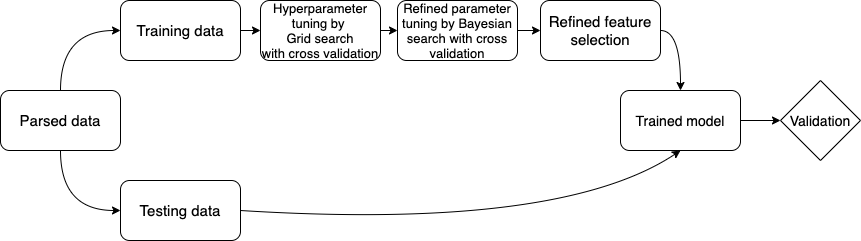
\includegraphics[width=1\linewidth]{training_validation}
		\label{fig:trainvalidationflowautoref}
		\caption{Flowchart of training a validation procedure for each of the two RF classifiers. We first use a grid search to obtain an initial guess of the model hyperparameters, we then refine our search using Bayesian hyperparameter selection with cross validation. Scoring function for the cross-validation is defined in Eq. \ref{eq:cvScore}. We then apply automatic selection of features based on the tuned model, and we train two classifiers to predict $\Delta S,\Delta C$. Validation is performed on $\sim10\%$ of the data.}
	\end{figure}
	\subsection{Hyper-parameter tuning }\label{subsection:hyperparameterTunning}
	To tune the parameters of the RF models, we first search for initial candidates using coarse grid search methodology with stratified cross-validation (CV). Using the initial values obtain by grid search we then refined the parameters using a Bayesian hyper-parameter tuning approach with CV step on the training data. To assure improvement in successive steps of CV, by which we wish to predict observations within the 0.25D error range, we design a specialized CV scoring function, $F_{cv}(\Delta)$ (Eq. \ref{eq:cvScore}) to be maximized, that is computed at the end of each iteration for both the coarse grid search and the Bayesian hyperparameter tuning, and is defined as follows:
	\beq\label{eq:cvScore}
	F_{cv}(\Delta) = \left(\sum_{i=1}^T\delta(\Delta )\right)e^{-\ds\sum_{i=1}^T H(0.25-|\Delta|)},
	\eeq 
	where $\Delta $ is the difference between registered subjective and predicted subjective  components of the refraction (for sphere or cylinder), $T$ is the number of training observations,  and $\delta$ is the delta function, defined as:
	\beqq
	\delta(x) = \begin{cases}
		1, & x=0;\\
		0,& x\neq 0,
	\end{cases}
	\eeqq 
	and $H(x)$ is the Heavyside function 
	\beqq
	H(x) = \begin{cases}
		1,& x\geq0;\\
		0,& \text{else}.
	\end{cases}
	\eeqq 
	The leading term in Eq. \ref{eq:cvScore} rewards exact prediction, whereas the exponential term penalizes CV scores for which the predicted $\Delta$ is larger than 0.25D. This promotes more observations to fall within the 0.25D error range. 
	The resulting parameters for both the $S$ and $C$ classifier appear in Table \ref{table:hyperparameters}.
	\begin{table}
		\begin{tabular}{c|c|c}
			Parameter & S & C\\
			\hline 
			Num. trees &755 & 254\\
			Criterion & gini& entropy\\
			Max. depth &45 & 51		
		\end{tabular}
		\caption{Optimized parameters for the sphere ($S$) and cylinder ($C$) Random-Forest classifiers.}
		\label{table:hyperparameters}
	\end{table}

	\section{Appendix}
	\subsection{Features selected}\label{subsection:featuresSelected}
	The following features were selected on an automatic model-based feature selection procedure. 
	For the Cylinder predictor we obtain the following features: 
	\begin{itemize}
		\item Age (years);
		\item objective cylinder in 3 and 5mm pupil radius;
		\item Zernike coefficient, $Z_2^{-2}$ (photo and meso);
		\item Zernike coefficient, $Z_4^0$ (photo and meso);  
		\item Zernike coefficient, $Z_3^1$ (photo and meso);
		\item White-to-white, $WTW$ (mm);
		\item Pachymetry ($\mu m$);
		\item kappa angle;
		\item Anterior Chamber Volume (ACV, see calculation in  subsection \ref{subsection:ACV});
		\item $ACD/P_r$, with $ACD$ the anterior chamber depth (mm) and $P_r$ the pupil radius (mm);
		\item  $P_r/WTW$;
		\item K-ratio $K2/K1$;
		\item $J0=-0.5C_o\cos(2A_o) $ for $P_r= 3mm$, where $A_o$ is the objective axis;
		\item $J45=-0.5C_o\sin(2A_o)$ for $P_r= 3mm$;
		\item Blur strength $\sqrt{M^2+J0^2 +J45^2}$, where $M= S_o+C_o/2$ is the spherical equivalent.
	\end{itemize}
	For the Sphere predictor we select the following features:
	\begin{itemize}
		\item Age (years); 
		\item Objective sphere ($P_r=3,5,7 mm$)
		\item Zernike coefficient $Z_2^{-2}$ (photo and meso);
		\item Zernike coefficient $Z_4^0$ (photo and meso);  
		\item Zernike coefficient $Z_3^1$ (photo and meso);
		\item Pupil radius $P_r$ (meso);
		\item Topo P value;
		\item Anterior chamber depth (ACD);
		\item Anterior Chamber Volume (ACV);
		\item white-to-white, $WTW$;
		\item kappa angle; 
		\item pachymetry ($\mu m$);
		\item $ACD/P_r$;
		\item  $P_r/WTW$;
		\item K-ratio $K2/K1$;
		\item $J0=-0.5C_o\cos(2A_o) $ for $P_r= 3mm$;
		\item $J45=-0.5C_o\sin(2A_o)$ for $P_r= 3mm$;
		\item Blur strength $\sqrt{M^2+J0^2 +J45^2}$, with $M= S_o+C_o/2$.
	\end{itemize}

    \subsection{Computation of the Anterior Chamber Volume}\label{subsection:ACV}
	The computation of the ACV relies on geometrical approximation, and is computed here in the following manner:
	First compute:
	\beqq 
	x      &=& \begin{cases}
		\sqrt{R^2 -\left(\frac{WTW}{2}\right)^2}, & R^2\geq \left(\frac{WTW}{2} \right)^2;\\
		0, \text{else},
	\end{cases}\\
	y      &=& R-ACD-x,\\
	v_Y &=& \frac{\pi y}{3}\left(\left(\frac{WTW}{2}\right)^2 + P_r^2 + \frac{WTWP_r}{2}\right),\\
	v_A &=&  \frac{\pi}{3}\left(\frac{3WTW}{2}- ACD-y\right)(ACD+y)^2,
	\eeqq
	where $R$ is the cornea radius (mm), $WTW$ is the white-to-white (mm), and $P_r$ is the pupil radius (mm).  
	Then compute 
	\beqq
	ACV = v_A-v_Y,
	\eeqq
	to obtain the anterior chamber volume ($mm^3$).

	
	\bibliographystyle{plain}
	\bibliography{ReportRxPrediction.bib}
	
\end{document}